	\chapter{ЗАДАЧА АВТОМАТИЗАЦИИ КОНФИГУРИРОВАНИЯ СЕТЕВОГО ОБОРУДОВАНИЯ}
	
	Специалистам, настраивающим оборудование Cisco, часто приходится использовать однообразные наборы команд конфигурации, порой отличающимися небольшим набором параметров, такими как IP-адрес устройства, идентификатор VLAN или диапазон IP-адресов при настройка DHCP.
	
	В связи с этим возникает задача автоматизировать процесс получения набора команд конфигурации, обеспечивающих следующий функционал:
	
	\begin{itemize}
		\item начальная настройка оборудования;
		\item настройка интерфейсов коммутатора/маршрутизатора;
		\item настройка VLAN'ов на коммутаторах;
		\item настройка DHCP на маршрутизаторах;
		\item настройка NAT на маршрутизаторах;
		\item настройка ACL(обычные и расширенные) на маршрутизаторах.
	\end{itemize}
	
	К программному обеспечению, решающему данную задачу, так же можно предъявить несколько требований:
	
	\begin{itemize}
		\item бесплатность;
		\item кроссплатформенность.
	\end{itemize} 
	
	Рассмотрим несколько приложений, позволяющих решить данную задачу.
%	
%	Сначала несколько слов по терминологии.
%	
%	Симуляторы — реализуют статичное множество команд, но, только
%	пользователь выходит за рамки возможного, выдают сообщение об ошибке. Классическим примером является Cisco Packet Tracer.
%	
%	Эмуляторы — дают возможность выполнять команды образов настоящих устройств, порой без заметных урезаний функциональности. Эмулятором, к примеру, является GNS3/Dynamips.
	
	\section{Cisco Packet Tracer}
	
	Packet Tracet  –-- официально выпускаемое Cisco
	программное обеспечение. Данный продукт доступен в версиях как для
	Windows, так и для Linux, бесплатно для учащихся Сетевой Академии
	Cisco.
	
	Интерфейс программы представлен на рисунке \ref{fig:packet_tracer}. Вся настройка осуществляется при помощи логической диаграммы сети.
	
	\begin{figure}[h!]
		\centering
		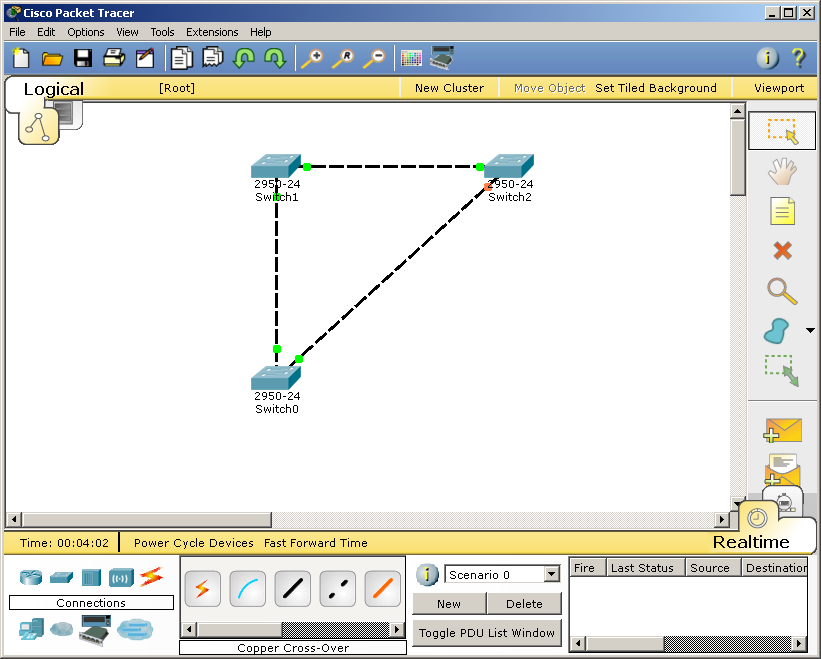
\includegraphics[width=0.9\linewidth]{pic/packet_tracer}
		\caption{Cisco Packet Tracer}
		\label{fig:packet_tracer}
	\end{figure}
	
	Достоинства Packet Tracer:
	
	\begin{itemize}
		\item дружественность и логичность интерфейса;
		\item доступность большого набора оборудования, выпускаемого Cisco;
		\item возможность перейти в режим симуляции и увидеть все действия с пакетами с использованием замедления времени.
	\end{itemize}
	
	Однако, поскольку Packet Tracer имитирует поведение оборудования Cisco, большинство действий по настройке производятся путем ввода необходимых команд в командную строку устройства, так же как если пользователь взаимодействовал бы с реальным оборудование.
	
	\section{GNS3}
	
	
	GNS3 (Graphical Network Simulator) --- представляет собой графический интерфейс, написанный на Qt, для эмулятора dynamips.
	
	Интерфейс программы продемонстрирован на рисунке \ref{fig:gns3}.
	GNS3 является свободно распространяемым проектом и доступен под следующими операционными системами: Linux, Windows и Mac OS X.
		
	\begin{figure}[h!]
		\centering
		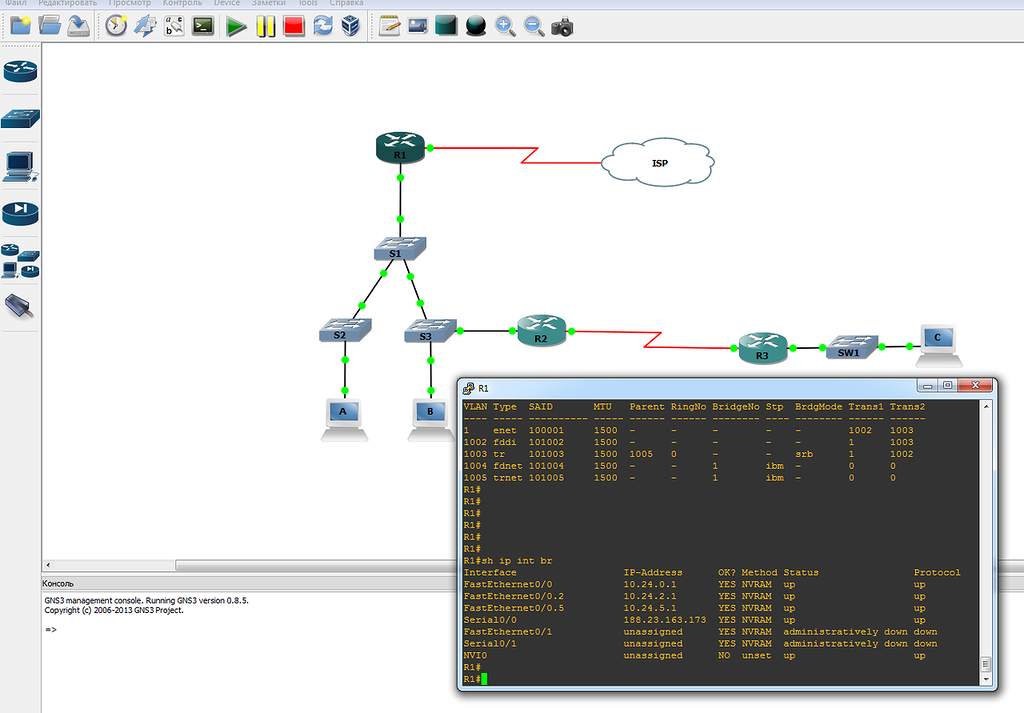
\includegraphics[width=0.9\linewidth]{pic/gns3}
		\caption{GNS3}
		\label{fig:gns3}
	\end{figure}
	
	GNS3 является эмулятором, который работает с оригинальными прошивками IOS.
	Это означает, что для использования GNS3, необходимо иметь в наличии реальные образы.
	
	Так же имеется ряд других недостатков:
	\begin{itemize}
		\item невозможность полноценно использовать коммутаторы;
		\item высокие требования к системным ресурсам;
		\item уменьшение производительности при увеличении количества устройств.
	\end{itemize}
		
	\section{Boson NetSim}
	
	Доступен в версии только для Windows, цена колеблется от 179\$ за CCNA и до 349\$ за CCNP.
	
	Выступает в роли набора лабораторных работ, объединенных по темам экзамена. Интерфейс разделен на нескольких разделов: постановка задачи, карта сети, в
	левой части находится список доступных лабораторных работ (в соответствии с рисунком \ref{fig:netsim}).
	
	После завершении выполнения лабораторной работы, можно получить результат и узнать, все ли было
	сделано.
	
	Присутствует возможность создания собственных топологий, с некоторыми
	ограничениями.
	
	
	\begin{figure}[h!]
		\centering
		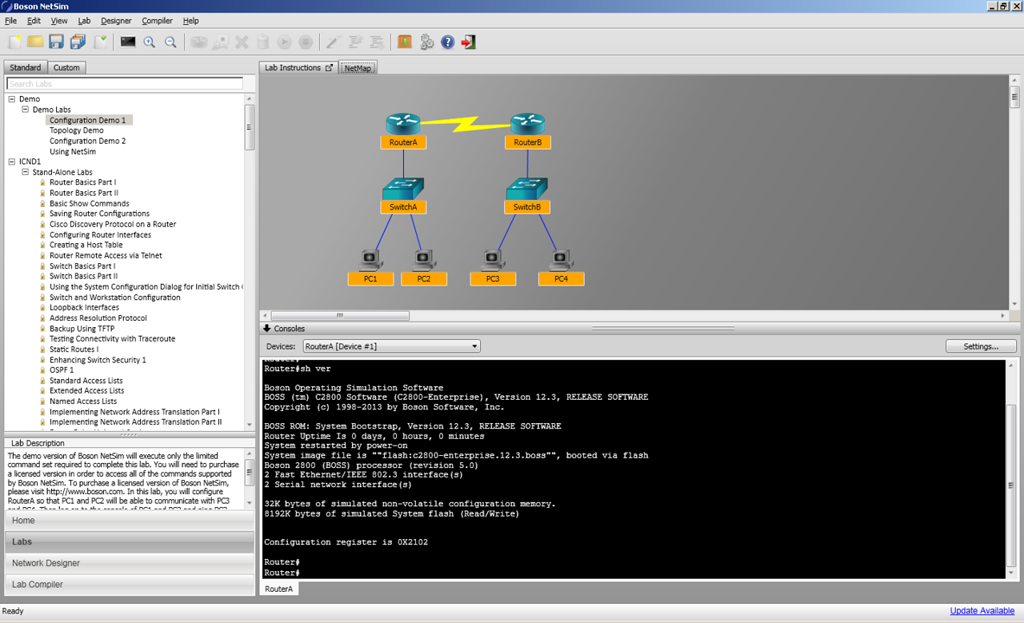
\includegraphics[width=0.9\linewidth]{pic/netsim}
		\caption{Boson NetSim}
		\label{fig:netsim}
	\end{figure}
	
	Ключевые возможности Boson NetSim:
	
	\begin{itemize}
		\item поддержка  42 маршрутизаторов, 6 коммутаторов;
		\item симуляция сетевого трафика при помощи технологии виртуальных
		пакетов;
		\item два режима просмотра: telnet или подключение по консоли;
		\item возможность создания собственных лабораторий.
	\end{itemize}
	
	\section{Cisco IOU}
	
	Последний в этом списке это  Cisco IOU (Cisco IOS on UNIX) —
	проприетарное ПО, которое официально не распространяется.
	
	Интерфейс программы представлен на рисунке \ref*{fig:ciscoIOU}.
	
	\begin{figure}[h!]
		\centering
		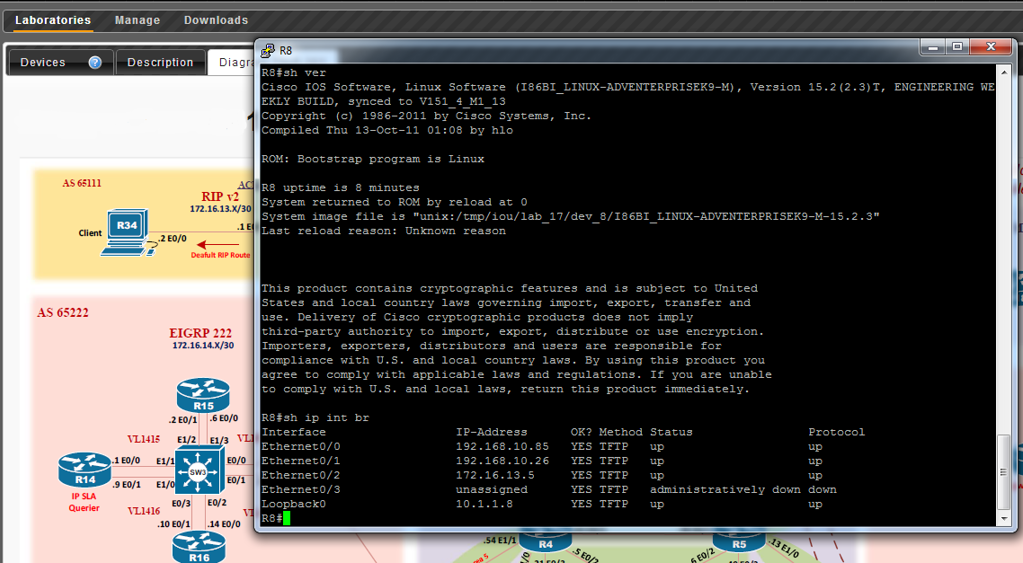
\includegraphics[width=0.9\linewidth]{pic/ciscoIOU}
		\caption{Cisco IOU}
		\label{fig:ciscoIOU}
	\end{figure}
	
	Существует мнение, что у Cisco есть возможность отследить и идентифицировать того, кто использует IOU.
	Известный факт состоит в том, что центр технической поддержки Cisco использует именно данных продукт.
	
	Сначала  был доступен только под Solaris, но затем был портирован и
	на Linux. В комплекте идут две основные части --- l2iou и l3iou. Первая часть эмулирует канальный уровень и коммутаторы, вторая же — сетевой уровень и маршрутизаторы.
	
	Настройка проводится путем редактирования конфигурационных файлов.%, недавно для него стал доступен также графический интерфейс.
	
%	Интерфейс довольно интуитивен, и позволяет выполнять почти все действия.
%	
%	В тоже время, включение на моделирование топологии, указанной на рис. \ref{fig:topologyCCIE}, приводит примерно к 50\% 	загрузке процессора.
%	
%	\begin{figure}[h!]
%		\centering
%		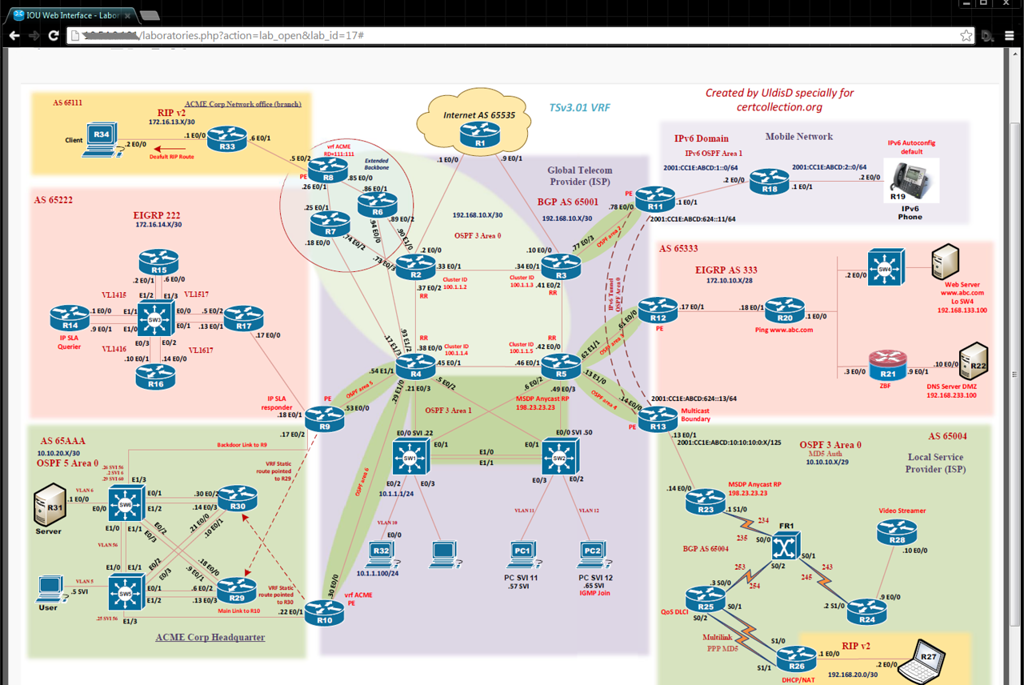
\includegraphics[width=0.7\linewidth]{pic/topologyCCIE}
%		\caption{Пример топологии}
%		\label{fig:topologyCCIE}
%	\end{figure}
%	
%	Надо сказать, данная топология предназначена для подготовки к сдаче экзамена на Cisco Certified Internetwork Expert.
%	
%	Возможности IOU на самом деле очень широкие. В тоже время, некоторые проблемы на канальном уровне все же имеются. Для некоторых устройств, например, отсутствует возможность жестко выставить дуплексный режим, но это всё мелочи.

	
	Сравнение рассмотренных программных продуктов приведено в таблице \ref{tab:econ_effect}.
	
	Общим недостатком представленных программных продуктов можно назвать излишнюю комплексность решения, вызванную попытками смоделировать полное поведение сетевых технологий. Это, в свою очередь, приводит к тому, графический интерфейс данных программ дает возможность пользователю построить логическую схему сети, но почти вся дальнейшая настройка, исключая, к примеру, название оборудования, производится путем ручного ввода соответствующих команд. И, как следствие,  отсутствует возможность шаблонизировать настройку требуемого функционала для дальнейшего использования на реальных устройствах.
	
	\begin{landscape}
		\begin{longtable}{|p{3.5cm}|p{5cm}|p{5cm}|p{5cm}|p{5cm}|} 
		% Вертикальная черта означает, что между полями должна быть вертикальная черта - разделитель
		% Заголовок таблицы на первой странице:
		\caption{Сравнение существующих решений\label{tab:econ_effect}}\\
		\hline % Вставляем горизонтальную линию
		{\centering Наименование показателей} & \centering Cisco Packet Tracer & \centering GNS3  & \centering Boson NetSim & Cisco IOU \\
		\hline
		\endfirsthead % Всё, что расположено выше считается заголовком таблицы и отображается на первой странице
		% Для второй и последующих страниц подменяем наименование таблицы в соответствии с требованиями:
		\caption*{Продолжение таблицы \ref{tab:econ_effect}}\\
		\hline
		\centering 1 & \centering 2 & \centering 3 \\
		\endhead % Всё что выше будет вставляться как заголовок на 2 и последующих страницах
		\hline
		
		Тип решения & симулятор & эмулятор & симулятор & симулятор \\
		\hline
		Ценовая политика & доступен студентам сетевой академии Cisco & бесплатен & от 179\$ за CCNA и до 349\$ за CCNP & проприетарен \\
		\hline
		Версии ОС & Windows, Linux & Linux, Windows и Mac OS X & Windows & Solaris, Linux \\

		\hline
	\end{longtable}
	
	
	
	\end{landscape}